\documentclass[]{article}
\usepackage{lmodern}
\usepackage{amssymb,amsmath}
\usepackage{ifxetex,ifluatex}
\usepackage{fixltx2e} % provides \textsubscript
\ifnum 0\ifxetex 1\fi\ifluatex 1\fi=0 % if pdftex
  \usepackage[T1]{fontenc}
  \usepackage[utf8]{inputenc}
\else % if luatex or xelatex
  \ifxetex
    \usepackage{mathspec}
  \else
    \usepackage{fontspec}
  \fi
  \defaultfontfeatures{Ligatures=TeX,Scale=MatchLowercase}
\fi
% use upquote if available, for straight quotes in verbatim environments
\IfFileExists{upquote.sty}{\usepackage{upquote}}{}
% use microtype if available
\IfFileExists{microtype.sty}{%
\usepackage{microtype}
\UseMicrotypeSet[protrusion]{basicmath} % disable protrusion for tt fonts
}{}
\usepackage[margin=1in]{geometry}
\usepackage{hyperref}
\hypersetup{unicode=true,
            pdftitle={Titanic Forever (Prediction Model for Survival with 84\% accuracy)},
            pdfauthor={Kshitiz Sirohi},
            pdfborder={0 0 0},
            breaklinks=true}
\urlstyle{same}  % don't use monospace font for urls
\usepackage{color}
\usepackage{fancyvrb}
\newcommand{\VerbBar}{|}
\newcommand{\VERB}{\Verb[commandchars=\\\{\}]}
\DefineVerbatimEnvironment{Highlighting}{Verbatim}{commandchars=\\\{\}}
% Add ',fontsize=\small' for more characters per line
\usepackage{framed}
\definecolor{shadecolor}{RGB}{248,248,248}
\newenvironment{Shaded}{\begin{snugshade}}{\end{snugshade}}
\newcommand{\KeywordTok}[1]{\textcolor[rgb]{0.13,0.29,0.53}{\textbf{#1}}}
\newcommand{\DataTypeTok}[1]{\textcolor[rgb]{0.13,0.29,0.53}{#1}}
\newcommand{\DecValTok}[1]{\textcolor[rgb]{0.00,0.00,0.81}{#1}}
\newcommand{\BaseNTok}[1]{\textcolor[rgb]{0.00,0.00,0.81}{#1}}
\newcommand{\FloatTok}[1]{\textcolor[rgb]{0.00,0.00,0.81}{#1}}
\newcommand{\ConstantTok}[1]{\textcolor[rgb]{0.00,0.00,0.00}{#1}}
\newcommand{\CharTok}[1]{\textcolor[rgb]{0.31,0.60,0.02}{#1}}
\newcommand{\SpecialCharTok}[1]{\textcolor[rgb]{0.00,0.00,0.00}{#1}}
\newcommand{\StringTok}[1]{\textcolor[rgb]{0.31,0.60,0.02}{#1}}
\newcommand{\VerbatimStringTok}[1]{\textcolor[rgb]{0.31,0.60,0.02}{#1}}
\newcommand{\SpecialStringTok}[1]{\textcolor[rgb]{0.31,0.60,0.02}{#1}}
\newcommand{\ImportTok}[1]{#1}
\newcommand{\CommentTok}[1]{\textcolor[rgb]{0.56,0.35,0.01}{\textit{#1}}}
\newcommand{\DocumentationTok}[1]{\textcolor[rgb]{0.56,0.35,0.01}{\textbf{\textit{#1}}}}
\newcommand{\AnnotationTok}[1]{\textcolor[rgb]{0.56,0.35,0.01}{\textbf{\textit{#1}}}}
\newcommand{\CommentVarTok}[1]{\textcolor[rgb]{0.56,0.35,0.01}{\textbf{\textit{#1}}}}
\newcommand{\OtherTok}[1]{\textcolor[rgb]{0.56,0.35,0.01}{#1}}
\newcommand{\FunctionTok}[1]{\textcolor[rgb]{0.00,0.00,0.00}{#1}}
\newcommand{\VariableTok}[1]{\textcolor[rgb]{0.00,0.00,0.00}{#1}}
\newcommand{\ControlFlowTok}[1]{\textcolor[rgb]{0.13,0.29,0.53}{\textbf{#1}}}
\newcommand{\OperatorTok}[1]{\textcolor[rgb]{0.81,0.36,0.00}{\textbf{#1}}}
\newcommand{\BuiltInTok}[1]{#1}
\newcommand{\ExtensionTok}[1]{#1}
\newcommand{\PreprocessorTok}[1]{\textcolor[rgb]{0.56,0.35,0.01}{\textit{#1}}}
\newcommand{\AttributeTok}[1]{\textcolor[rgb]{0.77,0.63,0.00}{#1}}
\newcommand{\RegionMarkerTok}[1]{#1}
\newcommand{\InformationTok}[1]{\textcolor[rgb]{0.56,0.35,0.01}{\textbf{\textit{#1}}}}
\newcommand{\WarningTok}[1]{\textcolor[rgb]{0.56,0.35,0.01}{\textbf{\textit{#1}}}}
\newcommand{\AlertTok}[1]{\textcolor[rgb]{0.94,0.16,0.16}{#1}}
\newcommand{\ErrorTok}[1]{\textcolor[rgb]{0.64,0.00,0.00}{\textbf{#1}}}
\newcommand{\NormalTok}[1]{#1}
\usepackage{graphicx,grffile}
\makeatletter
\def\maxwidth{\ifdim\Gin@nat@width>\linewidth\linewidth\else\Gin@nat@width\fi}
\def\maxheight{\ifdim\Gin@nat@height>\textheight\textheight\else\Gin@nat@height\fi}
\makeatother
% Scale images if necessary, so that they will not overflow the page
% margins by default, and it is still possible to overwrite the defaults
% using explicit options in \includegraphics[width, height, ...]{}
\setkeys{Gin}{width=\maxwidth,height=\maxheight,keepaspectratio}
\IfFileExists{parskip.sty}{%
\usepackage{parskip}
}{% else
\setlength{\parindent}{0pt}
\setlength{\parskip}{6pt plus 2pt minus 1pt}
}
\setlength{\emergencystretch}{3em}  % prevent overfull lines
\providecommand{\tightlist}{%
  \setlength{\itemsep}{0pt}\setlength{\parskip}{0pt}}
\setcounter{secnumdepth}{0}
% Redefines (sub)paragraphs to behave more like sections
\ifx\paragraph\undefined\else
\let\oldparagraph\paragraph
\renewcommand{\paragraph}[1]{\oldparagraph{#1}\mbox{}}
\fi
\ifx\subparagraph\undefined\else
\let\oldsubparagraph\subparagraph
\renewcommand{\subparagraph}[1]{\oldsubparagraph{#1}\mbox{}}
\fi

%%% Use protect on footnotes to avoid problems with footnotes in titles
\let\rmarkdownfootnote\footnote%
\def\footnote{\protect\rmarkdownfootnote}

%%% Change title format to be more compact
\usepackage{titling}

% Create subtitle command for use in maketitle
\newcommand{\subtitle}[1]{
  \posttitle{
    \begin{center}\large#1\end{center}
    }
}

\setlength{\droptitle}{-2em}

  \title{Titanic Forever (Prediction Model for Survival with 84\% accuracy)}
    \pretitle{\vspace{\droptitle}\centering\huge}
  \posttitle{\par}
    \author{Kshitiz Sirohi}
    \preauthor{\centering\large\emph}
  \postauthor{\par}
      \predate{\centering\large\emph}
  \postdate{\par}
    \date{January 7, 2019}


\begin{document}
\maketitle

\subsection{Introduction}\label{introduction}

Titanic dataset is famous for building a prediction model; whosoever
have started his/her journey into the field of Machine Learning would
know that. The dataset has 1309 observations and 12 variables. The
predciton that has to be made is that ``given certain set of variables,
predict that a pessanger would have survived or died''. Since we can
only have two value as output, this is a classification problem. Let's
get started.

\subsection{Loading packages}\label{loading-packages}

\begin{Shaded}
\begin{Highlighting}[]
\KeywordTok{library}\NormalTok{(ggplot2)}
\KeywordTok{library}\NormalTok{(dplyr)}
\end{Highlighting}
\end{Shaded}

\begin{verbatim}
## 
## Attaching package: 'dplyr'
\end{verbatim}

\begin{verbatim}
## The following objects are masked from 'package:stats':
## 
##     filter, lag
\end{verbatim}

\begin{verbatim}
## The following objects are masked from 'package:base':
## 
##     intersect, setdiff, setequal, union
\end{verbatim}

\begin{Shaded}
\begin{Highlighting}[]
\KeywordTok{library}\NormalTok{(randomForest)}
\end{Highlighting}
\end{Shaded}

\begin{verbatim}
## Warning: package 'randomForest' was built under R version 3.5.2
\end{verbatim}

\begin{verbatim}
## randomForest 4.6-14
\end{verbatim}

\begin{verbatim}
## Type rfNews() to see new features/changes/bug fixes.
\end{verbatim}

\begin{verbatim}
## 
## Attaching package: 'randomForest'
\end{verbatim}

\begin{verbatim}
## The following object is masked from 'package:dplyr':
## 
##     combine
\end{verbatim}

\begin{verbatim}
## The following object is masked from 'package:ggplot2':
## 
##     margin
\end{verbatim}

\subsection{Loading Data}\label{loading-data}

\begin{Shaded}
\begin{Highlighting}[]
\KeywordTok{setwd}\NormalTok{(}\StringTok{"C:/Users/ksiro/Documents/"}\NormalTok{)}
\NormalTok{t<-}\StringTok{ }\KeywordTok{read.csv}\NormalTok{(}\StringTok{"train.csv"}\NormalTok{,}\DataTypeTok{sep=}\StringTok{","}\NormalTok{,}\DataTypeTok{header=}\OtherTok{TRUE}\NormalTok{)}

\NormalTok{te <-}\StringTok{ }\KeywordTok{read.csv}\NormalTok{(}\StringTok{"test.csv"}\NormalTok{,}\DataTypeTok{sep=}\StringTok{","}\NormalTok{,}\DataTypeTok{header=}\OtherTok{TRUE}\NormalTok{)}
\NormalTok{te}\OperatorTok{$}\NormalTok{Survived <-}\StringTok{ }\OtherTok{NA}
\NormalTok{df<-}\KeywordTok{rbind}\NormalTok{(t,te)}
\NormalTok{df <-}\StringTok{ }\KeywordTok{as.data.frame}\NormalTok{(df)}
\end{Highlighting}
\end{Shaded}

\subsection{Understanding Data}\label{understanding-data}

This is how it looks after we load the data and combine them by rows.

\begin{Shaded}
\begin{Highlighting}[]
\KeywordTok{summary}\NormalTok{(df)}
\end{Highlighting}
\end{Shaded}

\begin{verbatim}
##   PassengerId      Survived          Pclass     
##  Min.   :   1   Min.   :0.0000   Min.   :1.000  
##  1st Qu.: 328   1st Qu.:0.0000   1st Qu.:2.000  
##  Median : 655   Median :0.0000   Median :3.000  
##  Mean   : 655   Mean   :0.3838   Mean   :2.295  
##  3rd Qu.: 982   3rd Qu.:1.0000   3rd Qu.:3.000  
##  Max.   :1309   Max.   :1.0000   Max.   :3.000  
##                 NA's   :418                     
##                                Name          Sex           Age       
##  Connolly, Miss. Kate            :   2   female:466   Min.   : 0.17  
##  Kelly, Mr. James                :   2   male  :843   1st Qu.:21.00  
##  Abbing, Mr. Anthony             :   1                Median :28.00  
##  Abbott, Mr. Rossmore Edward     :   1                Mean   :29.88  
##  Abbott, Mrs. Stanton (Rosa Hunt):   1                3rd Qu.:39.00  
##  Abelson, Mr. Samuel             :   1                Max.   :80.00  
##  (Other)                         :1301                NA's   :263    
##      SibSp            Parch            Ticket          Fare        
##  Min.   :0.0000   Min.   :0.000   CA. 2343:  11   Min.   :  0.000  
##  1st Qu.:0.0000   1st Qu.:0.000   1601    :   8   1st Qu.:  7.896  
##  Median :0.0000   Median :0.000   CA 2144 :   8   Median : 14.454  
##  Mean   :0.4989   Mean   :0.385   3101295 :   7   Mean   : 33.295  
##  3rd Qu.:1.0000   3rd Qu.:0.000   347077  :   7   3rd Qu.: 31.275  
##  Max.   :8.0000   Max.   :9.000   347082  :   7   Max.   :512.329  
##                                   (Other) :1261   NA's   :1        
##              Cabin      Embarked
##                 :1014    :  2   
##  C23 C25 C27    :   6   C:270   
##  B57 B59 B63 B66:   5   Q:123   
##  G6             :   5   S:914   
##  B96 B98        :   4           
##  C22 C26        :   4           
##  (Other)        : 271
\end{verbatim}

This is how top 6 values looks like in ``df'' data frame

\begin{Shaded}
\begin{Highlighting}[]
\KeywordTok{head}\NormalTok{(df)}
\end{Highlighting}
\end{Shaded}

\begin{verbatim}
##   PassengerId Survived Pclass
## 1           1        0      3
## 2           2        1      1
## 3           3        1      3
## 4           4        1      1
## 5           5        0      3
## 6           6        0      3
##                                                  Name    Sex Age SibSp
## 1                             Braund, Mr. Owen Harris   male  22     1
## 2 Cumings, Mrs. John Bradley (Florence Briggs Thayer) female  38     1
## 3                              Heikkinen, Miss. Laina female  26     0
## 4        Futrelle, Mrs. Jacques Heath (Lily May Peel) female  35     1
## 5                            Allen, Mr. William Henry   male  35     0
## 6                                    Moran, Mr. James   male  NA     0
##   Parch           Ticket    Fare Cabin Embarked
## 1     0        A/5 21171  7.2500              S
## 2     0         PC 17599 71.2833   C85        C
## 3     0 STON/O2. 3101282  7.9250              S
## 4     0           113803 53.1000  C123        S
## 5     0           373450  8.0500              S
## 6     0           330877  8.4583              Q
\end{verbatim}

This is how last 6 values looks like in ``df'' data frame

\begin{Shaded}
\begin{Highlighting}[]
\KeywordTok{tail}\NormalTok{(df)}
\end{Highlighting}
\end{Shaded}

\begin{verbatim}
##      PassengerId Survived Pclass                           Name    Sex
## 1304        1304       NA      3 Henriksson, Miss. Jenny Lovisa female
## 1305        1305       NA      3             Spector, Mr. Woolf   male
## 1306        1306       NA      1   Oliva y Ocana, Dona. Fermina female
## 1307        1307       NA      3   Saether, Mr. Simon Sivertsen   male
## 1308        1308       NA      3            Ware, Mr. Frederick   male
## 1309        1309       NA      3       Peter, Master. Michael J   male
##       Age SibSp Parch             Ticket     Fare Cabin Embarked
## 1304 28.0     0     0             347086   7.7750              S
## 1305   NA     0     0          A.5. 3236   8.0500              S
## 1306 39.0     0     0           PC 17758 108.9000  C105        C
## 1307 38.5     0     0 SOTON/O.Q. 3101262   7.2500              S
## 1308   NA     0     0             359309   8.0500              S
## 1309   NA     1     1               2668  22.3583              C
\end{verbatim}

If we check the 11th column , we can see that there are a lot of missing
values. So it makes sense to remove the whole column. So, after removing
the 11th coulmn we can see down below how many missing values each
coulmn in the table have.

\begin{Shaded}
\begin{Highlighting}[]
\NormalTok{df <-}\StringTok{ }\NormalTok{df[,}\OperatorTok{-}\DecValTok{11}\NormalTok{] ##removing the 11th column}

\NormalTok{m <-}\StringTok{ }\KeywordTok{as.data.frame}\NormalTok{(}\KeywordTok{matrix}\NormalTok{(}\DataTypeTok{ncol=}\DecValTok{1}\NormalTok{,}\DataTypeTok{nrow=}\DecValTok{1}\NormalTok{))   ##creating an empty data frame}
\ControlFlowTok{for}\NormalTok{ (i }\ControlFlowTok{in} \KeywordTok{c}\NormalTok{(}\DecValTok{1}\OperatorTok{:}\DecValTok{11}\NormalTok{)) \{ m[i]<-}\StringTok{ }\KeywordTok{sum}\NormalTok{(}\KeywordTok{is.na}\NormalTok{(df[,i])) \}   ## storting the values of number of missing values in data frame}
\NormalTok{m}
\end{Highlighting}
\end{Shaded}

\begin{verbatim}
##   V1  V2 V3 V4 V5  V6 V7 V8 V9 V10 V11
## 1  0 418  0  0  0 263  0  0  0   1   0
\end{verbatim}

Since we know how many NAs we have in each column, we now need to impute
those which actual values. In the summary below, we can check the mean,
median, min ,max of Age variable.

\begin{Shaded}
\begin{Highlighting}[]
\KeywordTok{summary}\NormalTok{(df}\OperatorTok{$}\NormalTok{Age)}
\end{Highlighting}
\end{Shaded}

\begin{verbatim}
##    Min. 1st Qu.  Median    Mean 3rd Qu.    Max.    NA's 
##    0.17   21.00   28.00   29.88   39.00   80.00     263
\end{verbatim}

After imputing we can see the change below.

\begin{Shaded}
\begin{Highlighting}[]
\NormalTok{df[}\KeywordTok{which}\NormalTok{(}\KeywordTok{is.na}\NormalTok{(df}\OperatorTok{$}\NormalTok{Age)),}\DecValTok{6}\NormalTok{] <-}\StringTok{ }\KeywordTok{mean}\NormalTok{(df}\OperatorTok{$}\NormalTok{Age,}\DataTypeTok{na.rm=}\OtherTok{TRUE}\NormalTok{)}
\KeywordTok{summary}\NormalTok{(df}\OperatorTok{$}\NormalTok{Age)}
\end{Highlighting}
\end{Shaded}

\begin{verbatim}
##    Min. 1st Qu.  Median    Mean 3rd Qu.    Max. 
##    0.17   22.00   29.88   29.88   35.00   80.00
\end{verbatim}

\textbf{Observation}

\begin{itemize}
\item
  column 6 has 263 NAs, so we need to impute some value. It can be mode,
  median or mean depending upon the situation. In our case, I have
  imputed mean because the mode and median are almost similar so it did
  not matter which one I use.
\item
  Column 2 also have 418 NAs but that is what we have to predict, so we
  do not bother filling it in.
\item
  I removed the cabin column since it had so many missing values.
\end{itemize}

\begin{center}\rule{0.5\linewidth}{\linethickness}\end{center}

Let's also impute values in Fare variable. We can see the summary of
fare down below. It has one NA, so after finding the index of that NA I
have imputed the value.

\begin{Shaded}
\begin{Highlighting}[]
\KeywordTok{summary}\NormalTok{(df}\OperatorTok{$}\NormalTok{Fare)}
\end{Highlighting}
\end{Shaded}

\begin{verbatim}
##    Min. 1st Qu.  Median    Mean 3rd Qu.    Max.    NA's 
##   0.000   7.896  14.454  33.295  31.275 512.329       1
\end{verbatim}

\begin{Shaded}
\begin{Highlighting}[]
\KeywordTok{which}\NormalTok{(}\KeywordTok{is.na}\NormalTok{(df}\OperatorTok{$}\NormalTok{Fare)) ## indexes are}
\end{Highlighting}
\end{Shaded}

\begin{verbatim}
## [1] 1044
\end{verbatim}

\begin{Shaded}
\begin{Highlighting}[]
\NormalTok{df}\OperatorTok{$}\NormalTok{Fare[}\DecValTok{1044}\NormalTok{] <-}\StringTok{ }\KeywordTok{median}\NormalTok{(df}\OperatorTok{$}\NormalTok{Fare,}\DataTypeTok{na.rm=}\OtherTok{TRUE}\NormalTok{)}
\end{Highlighting}
\end{Shaded}

The reason to impute median is that the variable fare has some outliers
which is skweing the mean value higher than median, which mean mean does
not represent the actual picture.

\begin{center}\rule{0.5\linewidth}{\linethickness}\end{center}

Imputing values in Embarked variable. We can see down below that one
element in embarked variables is empty space. So, I have found out the
index of it, that is 62 and 830 and imputed the values.

\begin{Shaded}
\begin{Highlighting}[]
\KeywordTok{table}\NormalTok{(df}\OperatorTok{$}\NormalTok{Embarked)            }
\end{Highlighting}
\end{Shaded}

\begin{verbatim}
## 
##       C   Q   S 
##   2 270 123 914
\end{verbatim}

\begin{Shaded}
\begin{Highlighting}[]
\KeywordTok{which}\NormalTok{(df}\OperatorTok{$}\NormalTok{Embarked}\OperatorTok{==}\StringTok{""}\NormalTok{)}
\end{Highlighting}
\end{Shaded}

\begin{verbatim}
## [1]  62 830
\end{verbatim}

\begin{Shaded}
\begin{Highlighting}[]
\NormalTok{df}\OperatorTok{$}\NormalTok{Embarked[}\KeywordTok{c}\NormalTok{(}\DecValTok{62}\NormalTok{,}\DecValTok{830}\NormalTok{)] <-}\StringTok{ "S"}
\NormalTok{df}\OperatorTok{$}\NormalTok{Embarked <-}\StringTok{ }\KeywordTok{droplevels}\NormalTok{(df}\OperatorTok{$}\NormalTok{Embarked)}
\KeywordTok{table}\NormalTok{(df}\OperatorTok{$}\NormalTok{Embarked)}
\end{Highlighting}
\end{Shaded}

\begin{verbatim}
## 
##   C   Q   S 
## 270 123 916
\end{verbatim}

\begin{itemize}
\tightlist
\item
  Above we can see that most of the time the embarked had value ``S'',
  that is why it makes sense to impute ``S'' in empty spaces whose index
  number we got from ``which'' function and used it to impute value.
\item
  We also had to drop the empty level, since it was a factor we only
  need those factor that hold some value.
\end{itemize}

\begin{center}\rule{0.5\linewidth}{\linethickness}\end{center}

We do not need passenger ID for the prediciton of survival because
unique ID cannot help in prediction.

\begin{Shaded}
\begin{Highlighting}[]
\NormalTok{##drop pasenger id}
\NormalTok{df <-}\StringTok{ }\NormalTok{df[,}\OperatorTok{-}\DecValTok{1}\NormalTok{]}
\end{Highlighting}
\end{Shaded}

\begin{center}\rule{0.5\linewidth}{\linethickness}\end{center}

In name column we are given full names of the passenger, I have taken
out only the title of their name so that we can predict does having a
higher title or lower title had any effect on the survival. Maybe higher
title are given higher prefference than people that hae lower title.
Take a look down below how many different titles we have.

\begin{Shaded}
\begin{Highlighting}[]
\NormalTok{##seprating title out of names in training}
\NormalTok{df}\OperatorTok{$}\NormalTok{Name <-}\StringTok{ }\KeywordTok{as.character}\NormalTok{(df}\OperatorTok{$}\NormalTok{Name)}
\NormalTok{lastname <-}\StringTok{ }\KeywordTok{strsplit}\NormalTok{(df}\OperatorTok{$}\NormalTok{Name,}\StringTok{","}\NormalTok{)}
\NormalTok{a <-}\StringTok{ }\KeywordTok{data.frame}\NormalTok{(}\KeywordTok{matrix}\NormalTok{(}\DataTypeTok{nrow=}\DecValTok{1}\NormalTok{,}\DataTypeTok{ncol=}\DecValTok{1}\NormalTok{))}
\NormalTok{a<-}\KeywordTok{as.list}\NormalTok{(a)}
\ControlFlowTok{for}\NormalTok{ (i }\ControlFlowTok{in} \KeywordTok{c}\NormalTok{(}\DecValTok{1}\OperatorTok{:}\KeywordTok{nrow}\NormalTok{(df))) \{ a[i] <-}\StringTok{ }\NormalTok{lastname[[i]][}\DecValTok{2}\NormalTok{]\}}
\NormalTok{a<-}\KeywordTok{as.character}\NormalTok{(a)}
\NormalTok{b <-}\StringTok{ }\KeywordTok{strsplit}\NormalTok{(a[}\DecValTok{1}\OperatorTok{:}\KeywordTok{nrow}\NormalTok{(df)],}\StringTok{". "}\NormalTok{)}
\NormalTok{title <-}\StringTok{ }\KeywordTok{data.frame}\NormalTok{(}\KeywordTok{matrix}\NormalTok{(}\DataTypeTok{ncol=}\DecValTok{1}\NormalTok{,}\DataTypeTok{nrow=}\DecValTok{1}\NormalTok{))}
\ControlFlowTok{for}\NormalTok{ (i }\ControlFlowTok{in} \KeywordTok{c}\NormalTok{(}\DecValTok{1}\OperatorTok{:}\KeywordTok{nrow}\NormalTok{(df))) \{ title [i] <-}\StringTok{ }\NormalTok{b[[i]][}\DecValTok{1}\NormalTok{]\}}
\NormalTok{title <-}\StringTok{ }\KeywordTok{trimws}\NormalTok{(title)}
\NormalTok{title <-}\StringTok{ }\KeywordTok{as.data.frame}\NormalTok{(title)}
\NormalTok{df <-}\StringTok{ }\KeywordTok{cbind}\NormalTok{(df,title)}
\NormalTok{df}\OperatorTok{$}\NormalTok{title <-}\StringTok{ }\KeywordTok{as.character}\NormalTok{(df}\OperatorTok{$}\NormalTok{title)}
\KeywordTok{table}\NormalTok{(df}\OperatorTok{$}\NormalTok{title)}
\end{Highlighting}
\end{Shaded}

\begin{verbatim}
## 
##     Capt      Col      Don     Dona       Dr Jonkheer     Lady    Major 
##        1        4        1        1        8        1        1        2 
##   Master     Miss     Mlle      Mme       Mr      Mrs       Ms      Rev 
##       61      260        2        1      757      197        2        8 
##      Sir       th 
##        1        1
\end{verbatim}

\begin{center}\rule{0.5\linewidth}{\linethickness}\end{center}

\subsection{Data Splitting}\label{data-splitting}

Now we are in the stage where have cleared the data. Now we can split
them back into training and testing. I split the data in two parts, one
part is ``df'' again, which holds training values, and another is
``test'' which holds test values.

\begin{Shaded}
\begin{Highlighting}[]
\NormalTok{test <-}\StringTok{ }\NormalTok{df[}\DecValTok{892}\OperatorTok{:}\StringTok{ }\DecValTok{1309}\NormalTok{,]}
\NormalTok{df <-}\StringTok{ }\NormalTok{df[}\DecValTok{1}\OperatorTok{:}\DecValTok{891}\NormalTok{,] ## I am strong training as df again}
\end{Highlighting}
\end{Shaded}

\begin{center}\rule{0.5\linewidth}{\linethickness}\end{center}

\subsection{Exploration}\label{exploration}

\textbf{Pclass vs survival}

Let's check out how does class variable affects the survival of the
passenger.

\begin{Shaded}
\begin{Highlighting}[]
\NormalTok{##most number of 3rd class passengers, almost half}
\KeywordTok{aggregate}\NormalTok{(df}\OperatorTok{$}\NormalTok{Survived,}\DataTypeTok{by=}\KeywordTok{list}\NormalTok{(df}\OperatorTok{$}\NormalTok{Pclass),}\DataTypeTok{FUN=}\NormalTok{mean) ##variying survival rate depending upon the class}
\end{Highlighting}
\end{Shaded}

\begin{verbatim}
##   Group.1         x
## 1       1 0.6296296
## 2       2 0.4728261
## 3       3 0.2423625
\end{verbatim}

\begin{Shaded}
\begin{Highlighting}[]
\KeywordTok{ggplot}\NormalTok{(df,}\KeywordTok{aes}\NormalTok{(}\DataTypeTok{x=}\NormalTok{Pclass,}\DataTypeTok{fill=}\KeywordTok{factor}\NormalTok{(Survived))) }\OperatorTok{+}\StringTok{ }\KeywordTok{geom_histogram}\NormalTok{(}\DataTypeTok{stat=}\StringTok{"count"}\NormalTok{)}
\end{Highlighting}
\end{Shaded}

\begin{verbatim}
## Warning: Ignoring unknown parameters: binwidth, bins, pad
\end{verbatim}

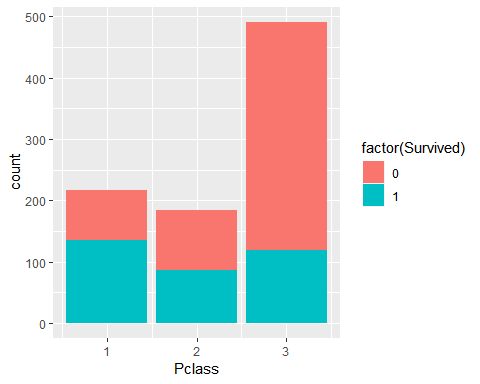
\includegraphics{Titanic_Survival_analysis_and_prediction_files/figure-latex/unnamed-chunk-14-1.pdf}
\textbf{Observations}

\begin{itemize}
\tightlist
\item
  Above we see that most of the passenger are from 3rd class category on
  ship.
\item
  In the plot we can see the survival rate of each one of those classes.
\end{itemize}

Also check out the pecentage of people survived in each category below.

\begin{Shaded}
\begin{Highlighting}[]
\CommentTok{#we see that people with high class had better chances of survival.}
\NormalTok{percent_survive_by_class <-}\StringTok{ }\NormalTok{df }\OperatorTok\StringTok{ }\KeywordTok{group_by}\NormalTok{(Pclass) }\OperatorTok\StringTok{ }\KeywordTok{summarise}\NormalTok{(}\DataTypeTok{survival_rate=}\KeywordTok{sum}\NormalTok{(Survived}\OperatorTok{==}\DecValTok{1}\NormalTok{)}\OperatorTok{*}\DecValTok{100}\OperatorTok{/}\StringTok{ }\NormalTok{(}\DataTypeTok{survival_rate=} \KeywordTok{sum}\NormalTok{(Survived }\OperatorTok{==}\DecValTok{1}\NormalTok{)}\OperatorTok{+}\KeywordTok{sum}\NormalTok{(Survived}\OperatorTok{==}\DecValTok{0}\NormalTok{)) )}
\NormalTok{percent_survive_by_class}
\end{Highlighting}
\end{Shaded}

\begin{verbatim}
## # A tibble: 3 x 2
##   Pclass survival_rate
##    <int>         <dbl>
## 1      1          63.0
## 2      2          47.3
## 3      3          24.2
\end{verbatim}

\textbf{Observations}

\begin{itemize}
\tightlist
\item
  We see that people from 1st class have higher rate of survival than
  people from 3rd class.
\end{itemize}

\begin{center}\rule{0.5\linewidth}{\linethickness}\end{center}

\textbf{Fare vs Survival}

Let's check how the fare variable affects the survival of passenger.

Here is the simple barplot of fare.

\begin{Shaded}
\begin{Highlighting}[]
\CommentTok{#sruvival vs fare}
\KeywordTok{barplot}\NormalTok{(df}\OperatorTok{$}\NormalTok{Fare)}
\end{Highlighting}
\end{Shaded}

\includegraphics{Titanic_Survival_analysis_and_prediction_files/figure-latex/unnamed-chunk-16-1.pdf}
I see a few outliers up there. Let's see the top 6 of those outliers
below.

\begin{Shaded}
\begin{Highlighting}[]
\NormalTok{fare <-}\StringTok{ }\KeywordTok{sort}\NormalTok{(df}\OperatorTok{$}\NormalTok{Fare,}\DataTypeTok{decreasing =}\NormalTok{ T)}
\KeywordTok{head}\NormalTok{(fare)}
\end{Highlighting}
\end{Shaded}

\begin{verbatim}
## [1] 512.3292 512.3292 512.3292 263.0000 263.0000 263.0000
\end{verbatim}

\begin{Shaded}
\begin{Highlighting}[]
\NormalTok{top_fare <-}\StringTok{ }\KeywordTok{tail}\NormalTok{(}\KeywordTok{order}\NormalTok{(df}\OperatorTok{$}\NormalTok{Fare),}\DecValTok{3}\NormalTok{)}
\NormalTok{df[top_fare,]}
\end{Highlighting}
\end{Shaded}

\begin{verbatim}
##     Survived Pclass                               Name    Sex Age SibSp
## 259        1      1                   Ward, Miss. Anna female  35     0
## 680        1      1 Cardeza, Mr. Thomas Drake Martinez   male  36     0
## 738        1      1             Lesurer, Mr. Gustave J   male  35     0
##     Parch   Ticket     Fare Embarked title
## 259     0 PC 17755 512.3292        C  Miss
## 680     1 PC 17755 512.3292        C    Mr
## 738     0 PC 17755 512.3292        C    Mr
\end{verbatim}

\begin{Shaded}
\begin{Highlighting}[]
\CommentTok{#all 3 with highest fare survived.}
\end{Highlighting}
\end{Shaded}

\textbf{Observations}

\begin{itemize}
\item
  I saw that there are few outliers in fare column. In the barplot above
  it can bee seen that three are above 500 and their are more that are
  higher than 200 but their quantity is very less in comparision to the
  whole dataset.
\item
  Above we can also see that all 3 passengers who paid 500 bucks have
  survived.
\end{itemize}

Let's analyse more on fare.

\begin{Shaded}
\begin{Highlighting}[]
\NormalTok{fare <-}\StringTok{ }\NormalTok{fare[}\OperatorTok{-}\KeywordTok{c}\NormalTok{(}\DecValTok{1}\NormalTok{,}\DecValTok{2}\NormalTok{,}\DecValTok{3}\NormalTok{)]}
\KeywordTok{head}\NormalTok{(fare)}
\end{Highlighting}
\end{Shaded}

\begin{verbatim}
## [1] 263.000 263.000 263.000 263.000 262.375 262.375
\end{verbatim}

\begin{Shaded}
\begin{Highlighting}[]
\KeywordTok{summary}\NormalTok{(fare)}
\end{Highlighting}
\end{Shaded}

\begin{verbatim}
##    Min. 1st Qu.  Median    Mean 3rd Qu.    Max. 
##   0.000   7.896  14.454  30.582  30.772 263.000
\end{verbatim}

\begin{Shaded}
\begin{Highlighting}[]
\KeywordTok{ggplot}\NormalTok{(df,}\KeywordTok{aes}\NormalTok{(Fare,}\DataTypeTok{color=}\KeywordTok{I}\NormalTok{(}\StringTok{"red"}\NormalTok{),}\DataTypeTok{fill=}\KeywordTok{I}\NormalTok{(}\StringTok{"green"}\NormalTok{),}\DataTypeTok{alpha=}\KeywordTok{I}\NormalTok{(}\FloatTok{0.3}\NormalTok{))) }\OperatorTok{+}\StringTok{ }\KeywordTok{geom_histogram}\NormalTok{(}\DataTypeTok{binwidth =} \DecValTok{1}\NormalTok{) }\OperatorTok{+}\StringTok{ }\KeywordTok{xlim}\NormalTok{(}\OtherTok{NA}\NormalTok{,}\DecValTok{50}\NormalTok{)}
\end{Highlighting}
\end{Shaded}

\begin{verbatim}
## Warning: Removed 160 rows containing non-finite values (stat_bin).
\end{verbatim}

\begin{verbatim}
## Warning: Removed 1 rows containing missing values (geom_bar).
\end{verbatim}

\includegraphics{Titanic_Survival_analysis_and_prediction_files/figure-latex/unnamed-chunk-18-1.pdf}

\begin{Shaded}
\begin{Highlighting}[]
\KeywordTok{ggplot}\NormalTok{(df,}\KeywordTok{aes}\NormalTok{(}\DataTypeTok{x=}\NormalTok{Fare,}\DataTypeTok{fill=}\KeywordTok{factor}\NormalTok{(Survived))) }\OperatorTok{+}\StringTok{ }\KeywordTok{geom_histogram}\NormalTok{()}\OperatorTok{+}\StringTok{ }\KeywordTok{xlim}\NormalTok{(}\DecValTok{0}\NormalTok{,}\DecValTok{100}\NormalTok{)}
\end{Highlighting}
\end{Shaded}

\begin{verbatim}
## `stat_bin()` using `bins = 30`. Pick better value with `binwidth`.
\end{verbatim}

\begin{verbatim}
## Warning: Removed 53 rows containing non-finite values (stat_bin).
\end{verbatim}

\begin{verbatim}
## Warning: Removed 4 rows containing missing values (geom_bar).
\end{verbatim}

\includegraphics{Titanic_Survival_analysis_and_prediction_files/figure-latex/unnamed-chunk-18-2.pdf}
\textbf{Observations}

\begin{itemize}
\item
  After removing the top three outliers, we can see that the mean value
  has changed. Not a very significant improvement but in some cases it
  can be significant.
\item
  In the one of the histogram above we can see that the most of the
  people paid between 5 to 30.
\item
  In the second chart above, we can see that higher the fare amount
  higher is the sruvival. That means people who paid maore were given
  more preference during emergency.
\end{itemize}

\begin{center}\rule{0.5\linewidth}{\linethickness}\end{center}

\textbf{Survival vs class}

\texttt{r\ \ \ ggplot(df,aes(x=Pclass,fill=factor(Survived)))\ +\ geom\_bar()}

\includegraphics{Titanic_Survival_analysis_and_prediction_files/figure-latex/unnamed-chunk-19-1.pdf}

\texttt{r\ \ \ percent\_survive\_by\_class\ \textless{}-\ df\ \%\textgreater{}\%\ group\_by(Pclass)\ \%\textgreater{}\%\ summarise(survival\_rate=sum(Survived==1)*100/\ (survival\_rate=\ sum(Survived\ ==1)+sum(Survived==0))\ )\ \ \ percent\_survive\_by\_class}

\texttt{\#\#\ \#\ A\ tibble:\ 3\ x\ 2\ \ \ \#\#\ \ \ Pclass\ survival\_rate\ \ \ \#\#\ \ \ \ \textless{}int\textgreater{}\ \ \ \ \ \ \ \ \ \textless{}dbl\textgreater{}\ \ \ \#\#\ 1\ \ \ \ \ \ 1\ \ \ \ \ \ \ \ \ \ 63.0\ \ \ \#\#\ 2\ \ \ \ \ \ 2\ \ \ \ \ \ \ \ \ \ 47.3\ \ \ \#\#\ 3\ \ \ \ \ \ 3\ \ \ \ \ \ \ \ \ \ 24.2}
\textbf{Observations}

\begin{itemize}
\tightlist
\item
  We see that people from 1st class have higher rate of survival than
  people from 3rd class.
\end{itemize}

\begin{center}\rule{0.5\linewidth}{\linethickness}\end{center}

\textbf{Survival vs Embarked}

\texttt{r\ \ \ ggplot(df,aes(x=Embarked,fill=factor(Survived)))\ +\ geom\_histogram(stat="count")}

\texttt{\#\#\ Warning:\ Ignoring\ unknown\ parameters:\ binwidth,\ bins,\ pad}

\includegraphics{Titanic_Survival_analysis_and_prediction_files/figure-latex/unnamed-chunk-20-1.pdf}

\texttt{r\ \ \ aggregate(df\$Survived,by=list(df\$Embarked),FUN=mean)}

\texttt{\#\#\ \ \ Group.1\ \ \ \ \ \ \ \ \ x\ \ \ \#\#\ 1\ \ \ \ \ \ \ C\ 0.5535714\ \ \ \#\#\ 2\ \ \ \ \ \ \ Q\ 0.3896104\ \ \ \#\#\ 3\ \ \ \ \ \ \ S\ 0.3390093}

\texttt{r\ \ \ \#\#\ there\ is\ sufficient\ difference\ in\ percentage,\ so\ we\ can\ use\ this\ also\ for\ prediction}
\textbf{Observations}

\begin{itemize}
\tightlist
\item
  In the table above we can see that only C has 55\% survival rate.
  Which can also be seen in the graph given after the table above.
\end{itemize}

\begin{center}\rule{0.5\linewidth}{\linethickness}\end{center}

\textbf{survival vs age} Let's see how does differece in age can make a
difference in the survival of a passenger.

\begin{Shaded}
\begin{Highlighting}[]
\KeywordTok{ggplot}\NormalTok{(df,}\KeywordTok{aes}\NormalTok{(}\DataTypeTok{x=}\NormalTok{Age)) }\OperatorTok{+}\StringTok{ }\KeywordTok{geom_density}\NormalTok{(}\DataTypeTok{col=}\StringTok{"green"}\NormalTok{,}\DataTypeTok{fill=}\StringTok{"red"}\NormalTok{,}\DataTypeTok{alpha=}\NormalTok{.}\DecValTok{4}\NormalTok{,}\DataTypeTok{size=}\DecValTok{1}\NormalTok{)}
\end{Highlighting}
\end{Shaded}

\includegraphics{Titanic_Survival_analysis_and_prediction_files/figure-latex/unnamed-chunk-21-1.pdf}

\begin{Shaded}
\begin{Highlighting}[]
\KeywordTok{ggplot}\NormalTok{(df,}\KeywordTok{aes}\NormalTok{(}\DataTypeTok{x=}\NormalTok{Age,}\DataTypeTok{fill=}\KeywordTok{factor}\NormalTok{(Survived))) }\OperatorTok{+}\StringTok{ }\KeywordTok{geom_histogram}\NormalTok{(}\DataTypeTok{binwidth =} \DecValTok{10}\NormalTok{)}
\end{Highlighting}
\end{Shaded}

\includegraphics{Titanic_Survival_analysis_and_prediction_files/figure-latex/unnamed-chunk-21-2.pdf}
\textbf{Observations}

\begin{itemize}
\tightlist
\item
  Most number of people on the ship was around 30 years of age. It can
  be seen in the plot above. There is a sudden spike in the density plot
  at age 30.
\item
  In the next plot we can see that as the age increased the survival
  rate also increassed. Meaning people that were either old or child,
  were given more preferences than middle age people during emergency.
\end{itemize}

\begin{center}\rule{0.5\linewidth}{\linethickness}\end{center}

\textbf{Sex vs survival}

\begin{Shaded}
\begin{Highlighting}[]
\KeywordTok{ggplot}\NormalTok{(df,}\KeywordTok{aes}\NormalTok{(}\DataTypeTok{x=}\NormalTok{Sex,}\DataTypeTok{fill=}\KeywordTok{factor}\NormalTok{(Survived))) }\OperatorTok{+}\StringTok{ }\KeywordTok{geom_histogram}\NormalTok{(}\DataTypeTok{stat=}\StringTok{"count"}\NormalTok{)}
\end{Highlighting}
\end{Shaded}

\begin{verbatim}
## Warning: Ignoring unknown parameters: binwidth, bins, pad
\end{verbatim}

\includegraphics{Titanic_Survival_analysis_and_prediction_files/figure-latex/unnamed-chunk-22-1.pdf}

\begin{Shaded}
\begin{Highlighting}[]
\NormalTok{## Women had higher survival rate}
\end{Highlighting}
\end{Shaded}

\textbf{Observations}

In the plot above we can see that women had higher survival rate,
meaning women were given preference during emergency.

\begin{center}\rule{0.5\linewidth}{\linethickness}\end{center}

\textbf{SibSp vs Survival}

Can having more number of siblings effects the chances of survival?

\begin{Shaded}
\begin{Highlighting}[]
\KeywordTok{ggplot}\NormalTok{(df,}\KeywordTok{aes}\NormalTok{(}\DataTypeTok{x=}\NormalTok{SibSp,}\DataTypeTok{fill=}\KeywordTok{factor}\NormalTok{(Survived))) }\OperatorTok{+}\StringTok{ }\KeywordTok{geom_bar}\NormalTok{(}\DataTypeTok{binwidth =}\NormalTok{ .}\DecValTok{5}\NormalTok{)}
\end{Highlighting}
\end{Shaded}

\begin{verbatim}
## Warning: `geom_bar()` no longer has a `binwidth` parameter. Please use
## `geom_histogram()` instead.
\end{verbatim}

\includegraphics{Titanic_Survival_analysis_and_prediction_files/figure-latex/unnamed-chunk-23-1.pdf}

\begin{Shaded}
\begin{Highlighting}[]
\NormalTok{##SURVIAL RATE DECREASSED AS THE RESPONSIBILITY INCREASED.}
\NormalTok{percent <-}\StringTok{ }\NormalTok{df }\OperatorTok\StringTok{ }\KeywordTok{group_by}\NormalTok{(SibSp) }\OperatorTok\StringTok{ }\KeywordTok{summarise}\NormalTok{(}\DataTypeTok{lived=}\KeywordTok{sum}\NormalTok{(Survived}\OperatorTok{==}\DecValTok{1}\NormalTok{),}\DataTypeTok{died=} \KeywordTok{sum}\NormalTok{(Survived}\OperatorTok{==}\DecValTok{0}\NormalTok{))}
\NormalTok{survival_rate <-}\StringTok{ }\NormalTok{(percent}\OperatorTok{$}\NormalTok{lived)}\OperatorTok{*}\DecValTok{100}\OperatorTok{/}\NormalTok{(percent}\OperatorTok{$}\NormalTok{lived }\OperatorTok{+}\StringTok{ }\NormalTok{percent}\OperatorTok{$}\NormalTok{died )}
\NormalTok{percent <-}\StringTok{ }\KeywordTok{cbind}\NormalTok{(percent,survival_rate)}
\NormalTok{percent}
\end{Highlighting}
\end{Shaded}

\begin{verbatim}
##   SibSp lived died survival_rate
## 1     0   210  398      34.53947
## 2     1   112   97      53.58852
## 3     2    13   15      46.42857
## 4     3     4   12      25.00000
## 5     4     3   15      16.66667
## 6     5     0    5       0.00000
## 7     8     0    7       0.00000
\end{verbatim}

\begin{Shaded}
\begin{Highlighting}[]
\KeywordTok{ggplot}\NormalTok{(percent,}\KeywordTok{aes}\NormalTok{(}\DataTypeTok{x=}\NormalTok{SibSp,}\DataTypeTok{y=}\NormalTok{survival_rate,}\DataTypeTok{col=}\KeywordTok{I}\NormalTok{(}\StringTok{"red"}\NormalTok{))) }\OperatorTok{+}\StringTok{ }\KeywordTok{geom_line}\NormalTok{()}
\end{Highlighting}
\end{Shaded}

\includegraphics{Titanic_Survival_analysis_and_prediction_files/figure-latex/unnamed-chunk-23-2.pdf}
\textbf{Observations}

\begin{itemize}
\tightlist
\item
  In percent table we can see that the survival rate is decreasing as
  the responsibility increase, by reponsibility I mean as the number of
  Siblings increased, in addition to spouses, the survival rate
  decreased.
\end{itemize}

\begin{center}\rule{0.5\linewidth}{\linethickness}\end{center}

\textbf{Parch vs Survival}

Can having more number of parents or chnidern means they had more
reponsibility and less chances of survival.

\begin{Shaded}
\begin{Highlighting}[]
\CommentTok{#having a parent or chind does not seem to efect the survial.}
\KeywordTok{ggplot}\NormalTok{(df,}\KeywordTok{aes}\NormalTok{(}\DataTypeTok{x=}\NormalTok{Parch,}\DataTypeTok{fill=}\KeywordTok{factor}\NormalTok{(Survived))) }\OperatorTok{+}\StringTok{ }\KeywordTok{geom_bar}\NormalTok{(}\DataTypeTok{binwidth =}\NormalTok{ .}\DecValTok{5}\NormalTok{)}
\end{Highlighting}
\end{Shaded}

\begin{verbatim}
## Warning: `geom_bar()` no longer has a `binwidth` parameter. Please use
## `geom_histogram()` instead.
\end{verbatim}

\includegraphics{Titanic_Survival_analysis_and_prediction_files/figure-latex/unnamed-chunk-24-1.pdf}

\begin{Shaded}
\begin{Highlighting}[]
\NormalTok{percent2 <-}\StringTok{ }\NormalTok{df }\OperatorTok\StringTok{ }\KeywordTok{group_by}\NormalTok{(Parch) }\OperatorTok\StringTok{ }\KeywordTok{summarise}\NormalTok{(}\DataTypeTok{lived=}\KeywordTok{sum}\NormalTok{(Survived}\OperatorTok{==}\DecValTok{1}\NormalTok{),}\DataTypeTok{died=} \KeywordTok{sum}\NormalTok{(Survived}\OperatorTok{==}\DecValTok{0}\NormalTok{))}
\NormalTok{survival_rate2 <-}\StringTok{ }\NormalTok{(percent2}\OperatorTok{$}\NormalTok{lived)}\OperatorTok{*}\DecValTok{100}\OperatorTok{/}\NormalTok{(percent2}\OperatorTok{$}\NormalTok{lived }\OperatorTok{+}\StringTok{ }\NormalTok{percent2}\OperatorTok{$}\NormalTok{died )}
\NormalTok{percent2 <-}\StringTok{ }\KeywordTok{cbind}\NormalTok{(percent2,survival_rate2)}
\NormalTok{percent2}
\end{Highlighting}
\end{Shaded}

\begin{verbatim}
##   Parch lived died survival_rate2
## 1     0   233  445       34.36578
## 2     1    65   53       55.08475
## 3     2    40   40       50.00000
## 4     3     3    2       60.00000
## 5     4     0    4        0.00000
## 6     5     1    4       20.00000
## 7     6     0    1        0.00000
\end{verbatim}

\begin{Shaded}
\begin{Highlighting}[]
\KeywordTok{ggplot}\NormalTok{(percent2,}\KeywordTok{aes}\NormalTok{(}\DataTypeTok{x=}\NormalTok{Parch,}\DataTypeTok{y=}\NormalTok{survival_rate2,}\DataTypeTok{col=}\KeywordTok{I}\NormalTok{(}\StringTok{"red"}\NormalTok{))) }\OperatorTok{+}\StringTok{ }\KeywordTok{geom_line}\NormalTok{()}
\end{Highlighting}
\end{Shaded}

\includegraphics{Titanic_Survival_analysis_and_prediction_files/figure-latex/unnamed-chunk-24-2.pdf}
\textbf{Observations}

\begin{itemize}
\tightlist
\item
  In the percent2 table above, we can see that there is not much
  variation in surivival rate depending upon the number of parent or
  child that individual have.
\item
  But, we can get a more clear picture if we combine SibSp and Parch and
  name it the whole family size. So let us do that.
\end{itemize}

\begin{center}\rule{0.5\linewidth}{\linethickness}\end{center}

\subsection{Introducing New Feature}\label{introducing-new-feature}

\textbf{Family size}

Let's create a new varibale called family size based on previous
varibales.

\begin{Shaded}
\begin{Highlighting}[]
\NormalTok{family_size <-}\StringTok{ }\NormalTok{df}\OperatorTok{$}\NormalTok{SibSp }\OperatorTok{+}\StringTok{ }\NormalTok{df}\OperatorTok{$}\NormalTok{Parch }\OperatorTok{+}\StringTok{ }\DecValTok{1}\NormalTok{      ##family size for training}
\NormalTok{df <-}\StringTok{ }\KeywordTok{cbind}\NormalTok{(df,family_size)}

\NormalTok{family_size <-}\StringTok{ }\NormalTok{test}\OperatorTok{$}\NormalTok{SibSp }\OperatorTok{+}\StringTok{ }\NormalTok{test}\OperatorTok{$}\NormalTok{Parch }\OperatorTok{+}\StringTok{ }\DecValTok{1}\NormalTok{    ##family size for test}
\NormalTok{test <-}\StringTok{ }\KeywordTok{cbind}\NormalTok{(test,family_size)}
\end{Highlighting}
\end{Shaded}

\textbf{Observations}

I have added the number of sibling and spouse to number of parents and
chinlders and 1 for the person itself. This can be a new feature called
family.

Creating the varibale for testing dataset too.

\begin{Shaded}
\begin{Highlighting}[]
\NormalTok{##family size for training set}
\KeywordTok{ggplot}\NormalTok{(df,}\KeywordTok{aes}\NormalTok{(}\DataTypeTok{x=}\NormalTok{family_size,}\DataTypeTok{fill=}\KeywordTok{factor}\NormalTok{(Survived))) }\OperatorTok{+}\StringTok{ }\KeywordTok{geom_bar}\NormalTok{(}\DataTypeTok{stat =} \StringTok{"count"}\NormalTok{)}
\end{Highlighting}
\end{Shaded}

\includegraphics{Titanic_Survival_analysis_and_prediction_files/figure-latex/unnamed-chunk-26-1.pdf}

\begin{Shaded}
\begin{Highlighting}[]
\NormalTok{percent3 <-}\StringTok{ }\NormalTok{df }\OperatorTok\StringTok{ }\KeywordTok{group_by}\NormalTok{(family_size) }\OperatorTok\StringTok{ }\KeywordTok{summarise}\NormalTok{(}\DataTypeTok{lived=}\KeywordTok{sum}\NormalTok{(Survived}\OperatorTok{==}\DecValTok{1}\NormalTok{),}\DataTypeTok{died=} \KeywordTok{sum}\NormalTok{(Survived}\OperatorTok{==}\DecValTok{0}\NormalTok{))}
\NormalTok{survival_rate3 <-}\StringTok{ }\NormalTok{(percent3}\OperatorTok{$}\NormalTok{lived)}\OperatorTok{*}\DecValTok{100}\OperatorTok{/}\NormalTok{(percent3}\OperatorTok{$}\NormalTok{lived }\OperatorTok{+}\StringTok{ }\NormalTok{percent3}\OperatorTok{$}\NormalTok{died )}
\NormalTok{percent3 <-}\StringTok{ }\KeywordTok{cbind}\NormalTok{(percent3,survival_rate3)}
\NormalTok{percent3}
\end{Highlighting}
\end{Shaded}

\begin{verbatim}
##   family_size lived died survival_rate3
## 1           1   163  374       30.35382
## 2           2    89   72       55.27950
## 3           3    59   43       57.84314
## 4           4    21    8       72.41379
## 5           5     3   12       20.00000
## 6           6     3   19       13.63636
## 7           7     4    8       33.33333
## 8           8     0    6        0.00000
## 9          11     0    7        0.00000
\end{verbatim}

\begin{Shaded}
\begin{Highlighting}[]
\KeywordTok{ggplot}\NormalTok{(percent3,}\KeywordTok{aes}\NormalTok{(}\DataTypeTok{x=}\NormalTok{family_size,}\DataTypeTok{y=}\NormalTok{survival_rate3,}\DataTypeTok{col=}\KeywordTok{I}\NormalTok{(}\StringTok{"red"}\NormalTok{))) }\OperatorTok{+}\StringTok{ }\KeywordTok{geom_line}\NormalTok{()}
\end{Highlighting}
\end{Shaded}

\includegraphics{Titanic_Survival_analysis_and_prediction_files/figure-latex/unnamed-chunk-26-2.pdf}
\textbf{Observations} * After calculating the total family size, I have
shown the survival rate in with respect to each category of family size.
* In second chart I have shown the trend of survival rate based on the
percentage of people survived belonging to each category.

Now to compare them all I have created a combined chart down below. *
(a) percent line chart that showed SibSp * (b) percent2 line chart that
showed Parch * (c) percent3 line chart that showed SibSp + Parch + 1

\begin{Shaded}
\begin{Highlighting}[]
\NormalTok{empty1 <-}\StringTok{ }\KeywordTok{data.frame}\NormalTok{(}\KeywordTok{matrix}\NormalTok{(}\KeywordTok{c}\NormalTok{(}\DecValTok{0}\NormalTok{,}\DecValTok{0}\NormalTok{,}\DecValTok{0}\NormalTok{,}\DecValTok{0}\NormalTok{,}\DecValTok{0}\NormalTok{,}\DecValTok{0}\NormalTok{,}\DecValTok{0}\NormalTok{,}\DecValTok{0}\NormalTok{),}\DataTypeTok{nrow=}\DecValTok{2}\NormalTok{,}\DataTypeTok{ncol=}\DecValTok{4}\NormalTok{))}
\NormalTok{empty2 <-}\StringTok{ }\KeywordTok{data.frame}\NormalTok{(}\KeywordTok{matrix}\NormalTok{(}\KeywordTok{c}\NormalTok{(}\DecValTok{0}\NormalTok{,}\DecValTok{0}\NormalTok{,}\DecValTok{0}\NormalTok{,}\DecValTok{0}\NormalTok{,}\DecValTok{0}\NormalTok{,}\DecValTok{0}\NormalTok{,}\DecValTok{0}\NormalTok{,}\DecValTok{0}\NormalTok{),}\DataTypeTok{nrow=}\DecValTok{2}\NormalTok{,}\DataTypeTok{ncol=}\DecValTok{4}\NormalTok{))}
\KeywordTok{colnames}\NormalTok{(empty1) <-}\StringTok{ }\KeywordTok{c}\NormalTok{(}\StringTok{"SibSp"}\NormalTok{, }\StringTok{"lived"}\NormalTok{, }\StringTok{"died"}\NormalTok{,}\StringTok{"survival_rate"}\NormalTok{)}
\KeywordTok{colnames}\NormalTok{(empty2) <-}\StringTok{ }\KeywordTok{c}\NormalTok{(}\StringTok{"Parch"}\NormalTok{, }\StringTok{"lived"}\NormalTok{, }\StringTok{"died"}\NormalTok{,}\StringTok{"survival_rate2"}\NormalTok{)}
\NormalTok{percent <-}\StringTok{ }\KeywordTok{rbind}\NormalTok{(percent,empty1)}
\NormalTok{percent2 <-}\StringTok{ }\KeywordTok{rbind}\NormalTok{(percent2,empty2)}
\NormalTok{dummy <-}\StringTok{ }\KeywordTok{cbind}\NormalTok{(percent[,}\KeywordTok{c}\NormalTok{(}\DecValTok{1}\NormalTok{,}\DecValTok{4}\NormalTok{)],percent2[,}\KeywordTok{c}\NormalTok{(}\DecValTok{1}\NormalTok{,}\DecValTok{4}\NormalTok{)], percent3[,}\KeywordTok{c}\NormalTok{(}\DecValTok{1}\NormalTok{,}\DecValTok{4}\NormalTok{)])}
\NormalTok{g <-}\StringTok{ }\KeywordTok{ggplot}\NormalTok{(dummy,}\KeywordTok{aes}\NormalTok{(}\DataTypeTok{x=}\NormalTok{family_size,}\DataTypeTok{y=}\NormalTok{survival_rate3,}\DataTypeTok{color=}\KeywordTok{I}\NormalTok{(}\StringTok{"red"}\NormalTok{),}\DataTypeTok{group=}\DecValTok{2}\NormalTok{)) }\OperatorTok{+}\StringTok{ }\KeywordTok{geom_line}\NormalTok{() ## after adding family}
\NormalTok{g <-}\StringTok{ }\NormalTok{g }\OperatorTok{+}\StringTok{ }\KeywordTok{geom_line}\NormalTok{(}\KeywordTok{aes}\NormalTok{(}\DataTypeTok{x=}\NormalTok{family_size,}\DataTypeTok{y=}\NormalTok{survival_rate2,}\DataTypeTok{color=}\StringTok{"green"}\NormalTok{)) }\OperatorTok{+}\StringTok{ }\KeywordTok{geom_point}\NormalTok{(}\DataTypeTok{shape=}\DecValTok{16}\NormalTok{)## only parent and child}
\NormalTok{g <-}\StringTok{ }\NormalTok{g }\OperatorTok{+}\StringTok{ }\KeywordTok{geom_line}\NormalTok{(}\KeywordTok{aes}\NormalTok{(}\DataTypeTok{x=}\NormalTok{family_size,}\DataTypeTok{y=}\NormalTok{survival_rate,}\DataTypeTok{color=}\StringTok{"blue"}\NormalTok{)) }\OperatorTok{+}\StringTok{ }\KeywordTok{geom_line}\NormalTok{() ## only spouse and siblings}
\NormalTok{g}
\end{Highlighting}
\end{Shaded}

\includegraphics{Titanic_Survival_analysis_and_prediction_files/figure-latex/unnamed-chunk-27-1.pdf}

\begin{center}\rule{0.5\linewidth}{\linethickness}\end{center}

\subsection{Changing features}\label{changing-features}

Below we can see that there are too many titles. So it is better to
merge some of them.

\begin{Shaded}
\begin{Highlighting}[]
\NormalTok{## survival vs title}
\KeywordTok{table}\NormalTok{(df}\OperatorTok{$}\NormalTok{title) }
\end{Highlighting}
\end{Shaded}

\begin{verbatim}
## 
##     Capt      Col      Don       Dr Jonkheer     Lady    Major   Master 
##        1        2        1        7        1        1        2       40 
##     Miss     Mlle      Mme       Mr      Mrs       Ms      Rev      Sir 
##      182        2        1      517      125        1        6        1 
##       th 
##        1
\end{verbatim}

Let's see how much percentage of people survived in each category of
title.

\begin{Shaded}
\begin{Highlighting}[]
\NormalTok{survival_by_title <-}\StringTok{ }\NormalTok{df }\OperatorTok\StringTok{ }\KeywordTok{group_by}\NormalTok{(title) }\OperatorTok\StringTok{ }\KeywordTok{summarise}\NormalTok{(}\DataTypeTok{value=}\KeywordTok{mean}\NormalTok{(Survived)}\OperatorTok{*}\DecValTok{100}\NormalTok{)}
\NormalTok{survival_by_title}
\end{Highlighting}
\end{Shaded}

\begin{verbatim}
## # A tibble: 17 x 2
##    title    value
##    <chr>    <dbl>
##  1 Capt       0  
##  2 Col       50  
##  3 Don        0  
##  4 Dr        42.9
##  5 Jonkheer   0  
##  6 Lady     100  
##  7 Major     50  
##  8 Master    57.5
##  9 Miss      69.8
## 10 Mlle     100  
## 11 Mme      100  
## 12 Mr        15.7
## 13 Mrs       79.2
## 14 Ms       100  
## 15 Rev        0  
## 16 Sir      100  
## 17 th       100
\end{verbatim}

Below is the visulization of title vs surivavl after merging the less
frequent titles.

\begin{Shaded}
\begin{Highlighting}[]
\NormalTok{df}\OperatorTok{$}\NormalTok{title[df}\OperatorTok{$}\NormalTok{title}\OperatorTok{!=}\StringTok{"Master"} \OperatorTok{&}\StringTok{ }\NormalTok{df}\OperatorTok{$}\NormalTok{title }\OperatorTok{!=}\StringTok{ "Miss"} \OperatorTok{&}\StringTok{ }\NormalTok{df}\OperatorTok{$}\NormalTok{title}\OperatorTok{!=}\StringTok{ "Mr"} \OperatorTok{&}\StringTok{ }\NormalTok{df}\OperatorTok{$}\NormalTok{title}\OperatorTok{!=}\StringTok{ "Mrs"}\NormalTok{] <-}\StringTok{ "Other"}
\KeywordTok{table}\NormalTok{(df}\OperatorTok{$}\NormalTok{title)}
\end{Highlighting}
\end{Shaded}

\begin{verbatim}
## 
## Master   Miss     Mr    Mrs  Other 
##     40    182    517    125     27
\end{verbatim}

\begin{Shaded}
\begin{Highlighting}[]
\KeywordTok{ggplot}\NormalTok{(df,}\KeywordTok{aes}\NormalTok{(}\DataTypeTok{x=}\NormalTok{title,}\DataTypeTok{fill=}\KeywordTok{factor}\NormalTok{(Survived))) }\OperatorTok{+}\StringTok{ }\KeywordTok{geom_bar}\NormalTok{()}
\end{Highlighting}
\end{Shaded}

\includegraphics{Titanic_Survival_analysis_and_prediction_files/figure-latex/unnamed-chunk-30-1.pdf}

Change title for test also.

\begin{Shaded}
\begin{Highlighting}[]
\NormalTok{test}\OperatorTok{$}\NormalTok{title[test}\OperatorTok{$}\NormalTok{title}\OperatorTok{!=}\StringTok{"Master"} \OperatorTok{&}\StringTok{ }\NormalTok{test}\OperatorTok{$}\NormalTok{title }\OperatorTok{!=}\StringTok{ "Miss"} \OperatorTok{&}\StringTok{ }\NormalTok{test}\OperatorTok{$}\NormalTok{title}\OperatorTok{!=}\StringTok{ "Mr"} \OperatorTok{&}\StringTok{ }\NormalTok{test}\OperatorTok{$}\NormalTok{title}\OperatorTok{!=}\StringTok{ "Mrs"}\NormalTok{] <-}\StringTok{ "Other"}
\end{Highlighting}
\end{Shaded}

\textbf{Observations}

\begin{itemize}
\tightlist
\item
  I have cahnged the feature named title. We can see that there are many
  different kind of title, then it makes sense to combine the less
  frequent ones together and let the more frequent ones as they are.
\item
  Then in the table we can see the title as well as their respective
  survival rate. We see that Womens are given most preference during
  emergency with Miss having 70\% survival and Mrs having 80\% survival
  rate.
\item
  Men with the tiel Mr., meaning an average man on the ship was given
  least preference.
\item
  We can also see it in the barplot above, where each title being
  presented with respective survival rate in blue.
\item
  Changing the title for test dataset also because the traning and
  testing dataset must have the consistency.
\end{itemize}

\begin{center}\rule{0.5\linewidth}{\linethickness}\end{center}

\subsection{Normalization}\label{normalization}

In classification problem, we need to normalize the countinous result so
that we can accomodate those continous variables between 0 and 1. To do
that, I have created a function called norm and then called fare and age
varible because they were continous. Both for testing and training
dataset.

\begin{Shaded}
\begin{Highlighting}[]
\NormalTok{##normalize continous variables}
\NormalTok{norm <-}\StringTok{ }\ControlFlowTok{function}\NormalTok{(x)\{(x}\OperatorTok{-}\KeywordTok{min}\NormalTok{(x))}\OperatorTok{/}\NormalTok{(}\KeywordTok{max}\NormalTok{(x)}\OperatorTok{-}\KeywordTok{min}\NormalTok{(x))\}}

\NormalTok{df}\OperatorTok{$}\NormalTok{Age<-}\StringTok{ }\KeywordTok{norm}\NormalTok{(df}\OperatorTok{$}\NormalTok{Age)}
\NormalTok{df}\OperatorTok{$}\NormalTok{Fare<-}\StringTok{  }\KeywordTok{norm}\NormalTok{(df}\OperatorTok{$}\NormalTok{Fare)}
\NormalTok{test}\OperatorTok{$}\NormalTok{Age<-}\StringTok{  }\KeywordTok{norm}\NormalTok{(test}\OperatorTok{$}\NormalTok{Age)}
\NormalTok{test}\OperatorTok{$}\NormalTok{Fare <-}\StringTok{ }\KeywordTok{norm}\NormalTok{(test}\OperatorTok{$}\NormalTok{Fare)}

\NormalTok{##subset only valuebale columns}
\NormalTok{train <-}\StringTok{ }\NormalTok{df[,}\KeywordTok{c}\NormalTok{(}\DecValTok{1}\NormalTok{,}\DecValTok{2}\NormalTok{,}\DecValTok{4}\NormalTok{,}\DecValTok{5}\NormalTok{,}\DecValTok{9}\NormalTok{,}\DecValTok{10}\NormalTok{,}\DecValTok{11}\NormalTok{,}\DecValTok{12}\NormalTok{)]}
\NormalTok{test <-}\StringTok{ }\NormalTok{test[,}\KeywordTok{c}\NormalTok{(}\DecValTok{1}\NormalTok{,}\DecValTok{2}\NormalTok{,}\DecValTok{4}\NormalTok{,}\DecValTok{5}\NormalTok{,}\DecValTok{9}\NormalTok{,}\DecValTok{10}\NormalTok{,}\DecValTok{11}\NormalTok{,}\DecValTok{12}\NormalTok{)]}
\end{Highlighting}
\end{Shaded}

\begin{center}\rule{0.5\linewidth}{\linethickness}\end{center}

Since we know we have a classification probelem at hand, it is
reasonable to convert evething into factor. Both for training and
testing dataset.

\begin{Shaded}
\begin{Highlighting}[]
\NormalTok{train}\OperatorTok{$}\NormalTok{Pclass <-}\StringTok{ }\KeywordTok{as.factor}\NormalTok{(train}\OperatorTok{$}\NormalTok{Pclass)}
\NormalTok{train}\OperatorTok{$}\NormalTok{title<-}\StringTok{ }\KeywordTok{as.factor}\NormalTok{(train}\OperatorTok{$}\NormalTok{title)}
\NormalTok{train}\OperatorTok{$}\NormalTok{Embarked <-}\StringTok{ }\KeywordTok{as.factor}\NormalTok{(df}\OperatorTok{$}\NormalTok{Embarked)}
\NormalTok{test}\OperatorTok{$}\NormalTok{Pclass <-}\StringTok{ }\KeywordTok{as.factor}\NormalTok{(test}\OperatorTok{$}\NormalTok{Pclass)}
\NormalTok{test}\OperatorTok{$}\NormalTok{title<-}\StringTok{ }\KeywordTok{as.factor}\NormalTok{(test}\OperatorTok{$}\NormalTok{title)}
\end{Highlighting}
\end{Shaded}

\begin{center}\rule{0.5\linewidth}{\linethickness}\end{center}

\subsection{Prediction}\label{prediction}

Use the random forest.

\begin{Shaded}
\begin{Highlighting}[]
\NormalTok{ramfor <-}\StringTok{ }\KeywordTok{randomForest}\NormalTok{( }\KeywordTok{factor}\NormalTok{(Survived) }\OperatorTok{~}\StringTok{ }\NormalTok{Pclass }\OperatorTok{+}\StringTok{ }\NormalTok{Sex }\OperatorTok{+}\StringTok{ }\NormalTok{Age }\OperatorTok{+}\StringTok{ }\NormalTok{Fare }\OperatorTok{+}\StringTok{ }\NormalTok{Embarked }\OperatorTok{+}\StringTok{ }\NormalTok{title }\OperatorTok{+}\StringTok{ }\NormalTok{family_size, }\DataTypeTok{data =}\NormalTok{ train)}
\NormalTok{ramfor}
\end{Highlighting}
\end{Shaded}

\begin{verbatim}
## 
## Call:
##  randomForest(formula = factor(Survived) ~ Pclass + Sex + Age +      Fare + Embarked + title + family_size, data = train) 
##                Type of random forest: classification
##                      Number of trees: 500
## No. of variables tried at each split: 2
## 
##         OOB estimate of  error rate: 16.72%
## Confusion matrix:
##     0   1 class.error
## 0 502  47   0.0856102
## 1 102 240   0.2982456
\end{verbatim}

\begin{Shaded}
\begin{Highlighting}[]
\KeywordTok{varImpPlot}\NormalTok{(ramfor)}
\end{Highlighting}
\end{Shaded}

\includegraphics{Titanic_Survival_analysis_and_prediction_files/figure-latex/unnamed-chunk-34-1.pdf}

\begin{Shaded}
\begin{Highlighting}[]
\NormalTok{pr <-}\StringTok{ }\KeywordTok{predict}\NormalTok{(ramfor,test)}
\end{Highlighting}
\end{Shaded}

\begin{center}\rule{0.5\linewidth}{\linethickness}\end{center}

By creating the confusion matrix we can determine how many false
positive and false negative we have. Moreover, we can also check the
accuracy of the result.

\begin{Shaded}
\begin{Highlighting}[]
\NormalTok{confusion_matrix <-}\StringTok{ }\NormalTok{ramfor[}\DecValTok{5}\NormalTok{]}
\NormalTok{confusion_matrix <-}\StringTok{ }\KeywordTok{as.data.frame}\NormalTok{(confusion_matrix)}
\NormalTok{Accuracy <-}\StringTok{ }\NormalTok{(confusion_matrix[}\DecValTok{1}\NormalTok{,}\DecValTok{1}\NormalTok{] }\OperatorTok{+}\StringTok{ }\NormalTok{confusion_matrix[}\DecValTok{2}\NormalTok{,}\DecValTok{2}\NormalTok{] )}\OperatorTok{/}\NormalTok{(confusion_matrix[}\DecValTok{1}\NormalTok{,}\DecValTok{2}\NormalTok{]}\OperatorTok{+}\NormalTok{confusion_matrix[}\DecValTok{2}\NormalTok{,}\DecValTok{2}\NormalTok{] }\OperatorTok{+}\NormalTok{confusion_matrix[}\DecValTok{2}\NormalTok{,}\DecValTok{1}\NormalTok{] }\OperatorTok{+}\NormalTok{confusion_matrix[}\DecValTok{1}\NormalTok{,}\DecValTok{1}\NormalTok{]  )}
\NormalTok{Accuracy <-}\StringTok{ }\KeywordTok{round}\NormalTok{(Accuracy,}\DecValTok{2}\NormalTok{)}
\KeywordTok{print}\NormalTok{(}\KeywordTok{paste}\NormalTok{(}\StringTok{"Accuracy is"}\NormalTok{, Accuracy}\OperatorTok{*}\DecValTok{100}\NormalTok{,}\StringTok{"%"}\NormalTok{))}
\end{Highlighting}
\end{Shaded}

\begin{verbatim}
## [1] "Accuracy is 83 %"
\end{verbatim}


\end{document}
